% \subsection{Overview}
% \label{subsec:method_overview}

% In this section, we introduce a new compositional architecture for orchestrating multiple SLMs and discuss its optimization. 


% Firstly, to address the challenge mentioned in Section~\ref{sect:failure}, we introduce a simple yet effective architecture that integrates models through a protocol-based mechanism (Section~\ref{sub:method-arch}). Based on this architecture, we introduce strategies to optimize \NAME{}{} from two directions: From the model perspective, we introduce model selection search to identify the most appropriate model to invoke within the \NAME{}{} (Section~\ref{sub:method-search}). From the test-time compute perspective, we explore optimal way compute scaling for the \NAME{}{} with searched model selections (Section~\ref{sec:scaling}). 

In this work, we set out to ask two critical questions: given a pool of available SLMs, how can we (i) orchestrate their outputs to achieve the best overall performance, and (ii) select an effective subset of models that maximizes accuracy?

To answer question (i), we present the \NAME{}{} (Section~\ref{sub:method-arch}), a simple yet effective orchestration method. To answer question (ii), we propose model selection search (Section~\ref{sub:method-search}) that identifies complementary subsets from dozens of available SLMs. Finally, we explore compute scaling strategies (Section~\ref{sec:scaling}) to further enhance the reasoning accuracy. 


% Specifically, we search for model compositions that maximize overall accuracy by exploiting complementary model abilities. Not all compositions are equally useful, for example, if one model is consistently stronger and already covers all the capabilities of a weaker model, then combining them will yield little gain. As a result, identifying orthogonal strengths is essential for constructing effective ensembles.

\subsection{\NAME{}{} for Orchestrating Multiple Small Language Models
}
\label{sub:method-arch}

% Based on analysis in Section~\ref{sect:failure}, we here propose a compositional architecture designed for SLMs. The underlying intuition can be illustrated with a simple analogy: 

% Suppose we pose the same question to two people. We can't discuss or ask additional questions to them after they answer. We don't know the knowledge to verify the answer. The first person responds with confidence, and the answer is highly consistent. The second person, in contrast, provides a self-contradicting answer. Which person should we trust? Intuitively, one would place more confidence in the first person, while regarding the second as less reliable. 

% Existing composition methods are typically developed for frontier models such as GPT-4o and rely on iterative, text-based discussion among models. However, in practice these interactions often amplify mistakes rather than correct them, leading to degraded accuracy. On the other hand, a simple voting strategy also performs suboptimally. Different models have distinct strengths and weaknesses: one model may give stable and consistent answers, while another may produce highly variable responses. Direct voting neutralizes the contribution of more reliable models.


% As shown in Figure~\ref{fig:small-large-accuracy}, existing methods often fail to surpass the accuracy of the best single model in the ensemble, motivating the need for a more principled architecture for small-scale models.



% We apply the same principle to SLMs. We let multiple SLMs first generate answers to a query, and then the final output is selected from the answer of the most confident model. We termed our method \textbf{\NAME{}{}}, which operates in two phase.

At a high level, our intuition is that we do not need to let SLMs discuss with each other. Instead, we can develop a simple rule-based method that estimates the confidence of each model’s answer and then selects the final output from the model with the highest confidence. We term our method \textbf{\NAME{}{}}, which operates in two phases.

\textbf{Independent Generation Phase.} For a given question, we first let each SLM independently generate multiple candidate responses to the same query prompt with temperature $>0$, producing a pool of sampled answers per model.

\looseness=-1
\textbf{Confidence Estimation Phase.} We evaluate the confidence of each SLM’s outputs by measuring their consistency across their own outputs. Intuitively, a model that places higher probability mass on the correct answer will reproduce the same answer across samples, whereas an uncertain model will scatter its outputs. For instance, if SLM A produces three identical answers while model B produces three different ones, the answer from model A is selected. This correlation between consistency and correctness is observed by previous papers.~\citep{wang2023selfconsistencyimproveschainthought,xie2024calibratingreasoninglanguagemodels,Taubenfeld_2025,chen2023universalselfconsistencylargelanguage} 

In cases where two SLMs are equally consistent but disagree, we use their validation accuracy as a tie-breaker. Prior work has shown that consistency is strongly correlated with correctness, which provides a rationale for this design.

For more details, Algorithm~\ref{alg:SLM-Mux} summarizes the workflow step by step. Figure~\ref{fig:SLM-Mux-method} provides a visual example of the workflow. The evaluation of \NAME{}{} is presented in Section~\ref{sub:vanilla}.

% The number of models and samples per model can be flexibly adjusted. Increasing the number of samples typically improves the confidence of consistency estimation. 

\begin{figure}[t]
  \centering
  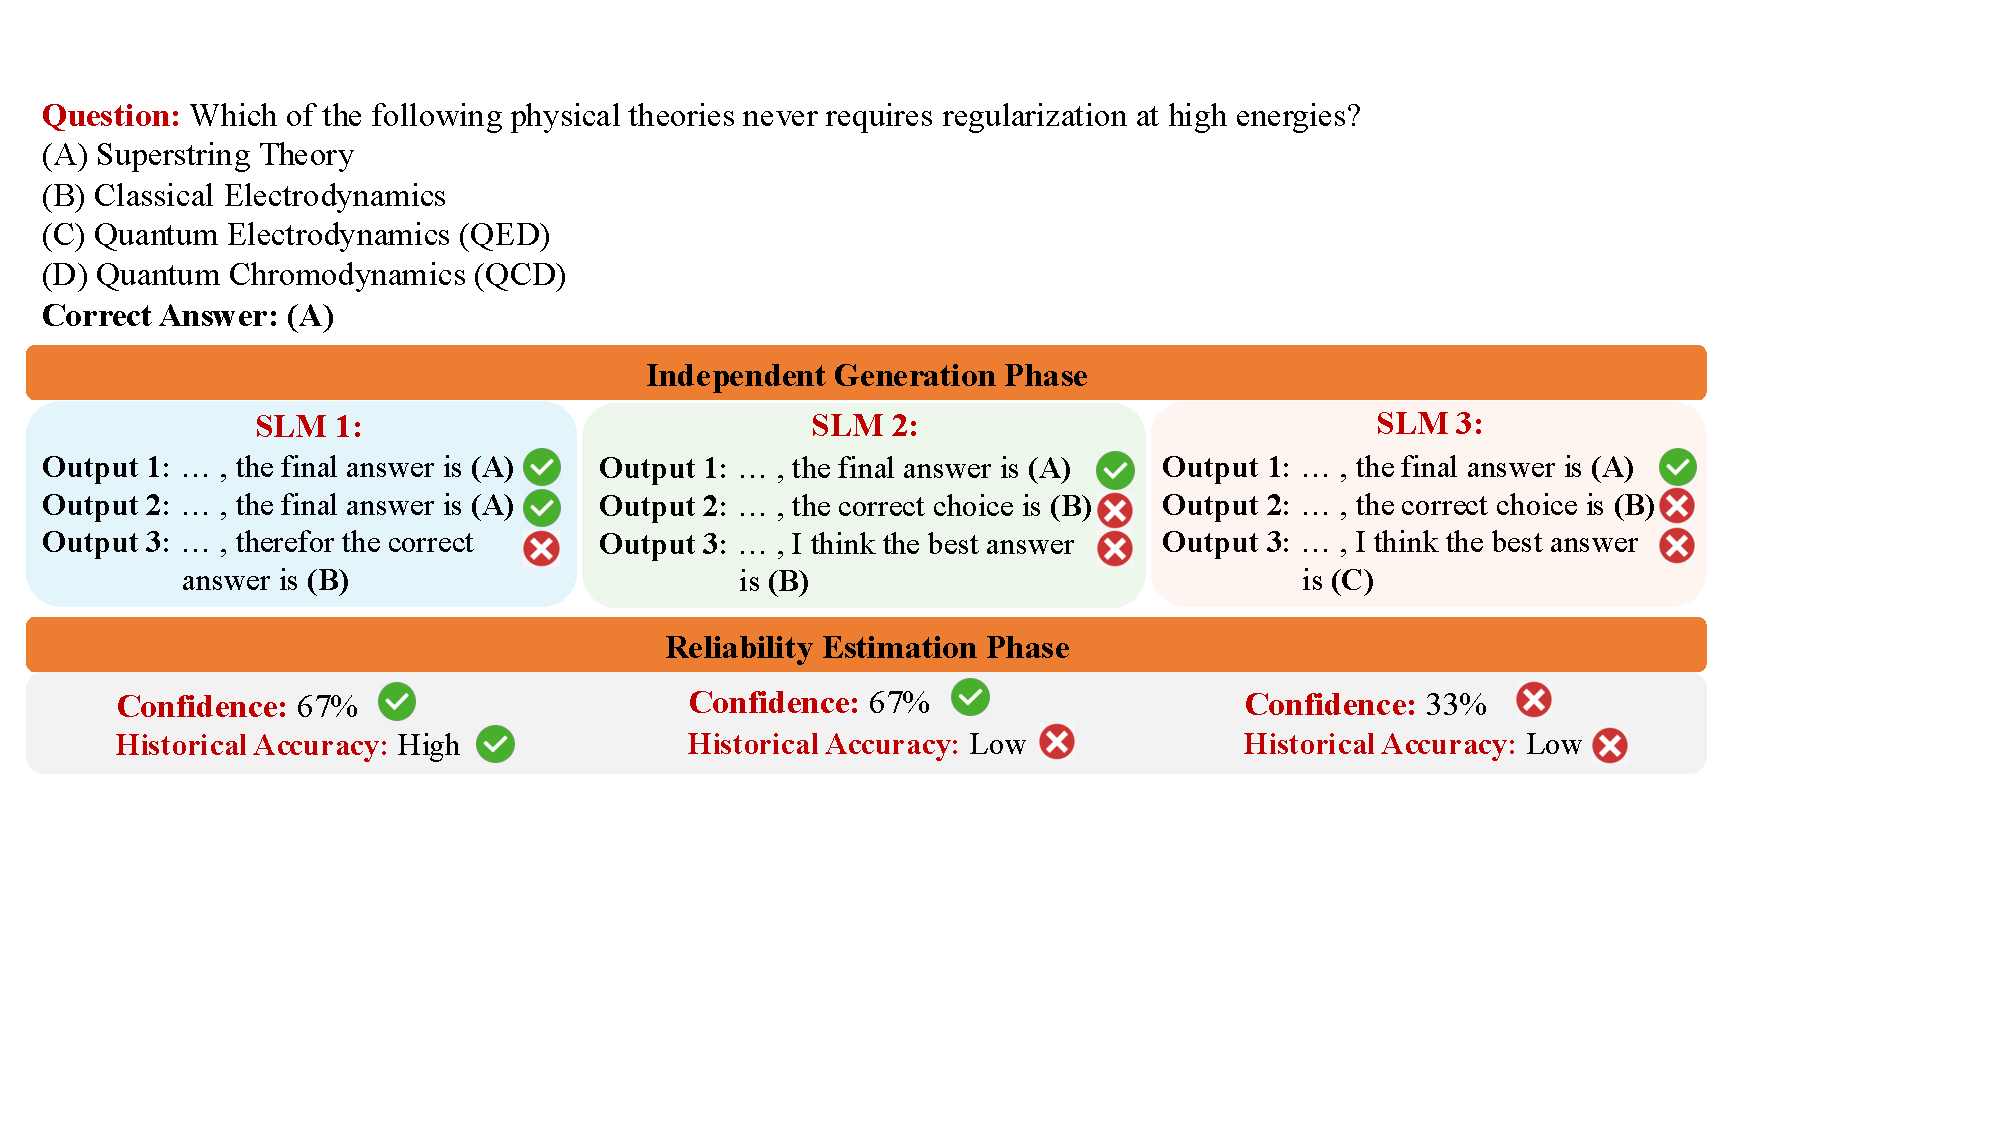
\includegraphics[width=\linewidth]{Figures/LM-Mux_workflow_v2.pdf}
  \vspace{-12pt}
  \caption{\small \textbf{Illustration of \NAME{}{} Workflow.}
(1) Each SLM first independently generates multiple outputs for the same question.
(2) The most frequent answer from each SLM is selected, and its frequency in the answer pool is used as the confidence score.
(3) The answers with the highest confidence score are selected.
(4) If multiple answers share the same confidence score, the tie is broken by selecting the answer from the SLM with the highest accuracy on the validation set. }
  \label{fig:SLM-Mux-method}
  \vspace{-20pt}
\end{figure}
% The inspiration behind our proposed approach stems from observing human problem-solving behaviors. When multiple individuals independently attempt to solve the same complex problem but are unable to communicate directly, selecting the most reliable answer becomes challenging~\cite{Condorcet1994}. Humans naturally employ metacognitive abilities, reflecting on their own responses to judge confidence~\cite{Flavell1979}. However, LLMs lack such ability and tend to exhibit overconfidence when self-assessing the accuracy of their outputs, making direct confidence querying not reliable and ineffective~\cite{geng2024surveyconfidenceestimationcalibration,yang2024trustllmsmitigateoverconfidence}. Motivated by previous works on model ensemble~\cite{gal2016dropoutbayesianapproximationrepresenting,lakshminarayanan2017simplescalablepredictiveuncertainty,wang2023selfconsistencyimproveschainthought}, we consider an alternative method: independently generating multiple samples from each model and then evaluating answer confidence based on the dispersion of these samples. By analyzing the distribution of independently generated answers and considering historical model performance metrics, we aim to reliably identify the most credible answer without explicit model self-assessment.



% By explicitly defining and enforcing aggregation protocols independent of textual interactions, we observe that \NAME{}{} method mitigates the superficial interaction issues common in traditional composition methods when applied to smaller-scale models.

\begin{figure}[t]
\begin{minipage}{\linewidth}
% \small
\begin{algorithm}[H]
\caption{\NAME{}{} Working Flow}
\label{alg:SLM-Mux}
\textbf{Input}: Models $M_1,\dots,M_n$, query $x$, samples per model $k$, validation accuracies $a_1,\dots,a_n$ \\
\textbf{Output}: Final answer $\hat{y}$
\begin{algorithmic}[1]
\Statex \textit{Independent Generation: each model produces multiple candidate answers independently}
\For{$i=1,\dots,n$}
    \State Sample $k$ answers $Y_i=\{y_i^{(1)},\dots,y_i^{(k)}\}$ from $M_i$
    \State Compute $f_i(y)=\tfrac{1}{k}\sum_{j=1}^{k}\mathbf{1}\!\left(y_i^{(j)}=y\right)$
    \State Let $y_i^*=\arg\max_{y} f_i(y)$ and set $s_i = f_i(y_i^*)$
\EndFor

\Statex \textit{Confidence Estimation: measure self-consistency and break ties by validation accuracy}
\State $S_{\max}=\max_{i} s_i$, \quad $I^*=\{\, i \mid s_i = S_{\max} \,\}$
\If{$|I^*|=1$}
    \State $i^* \gets \text{the unique index in } I^*$
\Else
    \State $i^* \gets \arg\max_{i \in I^*} a_i$
\EndIf
\State \textbf{return} $\hat{y}=y_{i^*}^*$
\end{algorithmic}
\end{algorithm}
\end{minipage}
\vspace{-5pt}
\end{figure}










% \begin{figure}[t]
%   \centering
%   \includegraphics[width=0.85\linewidth]{Figures/\NAME{}{}_workflow.pdf}
%   % \vspace{-5pt}
%   \caption{\small \textbf{Illustration of \NAME{}{} Workflow.}
% Detailed workflow of the proposed \NAME{}{} method. 
% (1) Each small language model independently generates multiple outputs from a straightforward, isolated prompt.
% (2) Responses are aggregated, and answer frequencies within each model are computed to establish a confidence score.
% (3) For tasks with finite answer spaces, responses meeting or exceeding a confidence threshold (e.g., 2/3 majority) are combined into a candidate pool.
% (4) Final selection from this pool leverages historical accuracy metrics of individual models to choose the most reliable answer.
%   }
%   \label{fig:SLM-Mux-method}
%   \vspace{-15pt}
% \end{figure}

% \vspace{-5pt}
\vspace{5pt}
\subsection{Model Selection Search for SLM-MUX Optimization}
% \vspace{3pt}
% \vspace{-3pt}
\label{sub:method-search}

% \paragraph{Intuition} In Section~\ref{sub:method-arch}, we introduced a new compositional architecture. A key question remains: which SLMs should be chosen to use in the architecture? With dozens of SLMs now available, we have access to a large model pool. Since it is not feasible to invoke every SLM in the \NAME{}{} for every given query, it is worth investigating whether there is an optimal strategy for selecting a limited subset of models for each task.
% 
% \subsubsection{Model Selection Optimization}
% \label{subsub: search}
% 
% Another motivation of model selection search is that for each task, choosing SLMs with overlapping strengths may bring little improvement, but selecting those with complementary strengths may significantly boost accuracy. For example, as shown in Figure~\ref{fig:motivation-search}, the models on the left have highly overlapping capabilities. Llama 3.2 3B offers no advantage in every subject: for most (if not all) MATH questions, if Qwen 2.5 7B cannot solve them, neither can Llama 3.2 3B. In this case, combining them provides no benefit. However, the models on the right show complementary strengths: Mistral Small 24B scores higher in some subjects, and Qwen 2.5 7B does better in others. In this case, when Qwen 2.5 7B cannot answer a question, Mistral Small 24B may succeed.
% 

At a high level, the idea of model selection search is to identify complementarity among models. The goal is not simply to add more models, but to bring new capabilities as we add models. To illustrate, Figure~\ref{fig:motivation-search} illustrates this intuition: Qwen2.5-7B consistently outperforms Llama3.2-3B across all subjects, so combining them offers no capability beyond what Qwen2.5-7B already provides. In contrast, Mistral Small 24B and Qwen2.5-7B show complementary strengths—one performs better in certain subjects while the other excels in different ones—so pairing them leads to clear gains.


We frame model selection as a search on the validation set with two competing objectives. Our search objective is formulated as follows:


% 

Our first objective is \textbf{Union Accuracy}, which reflects the overall accuracy 
of the system. The higher the union accuracy is, the more questions a system can potentially answer. Formally, let 
$\mathcal{M} = \{m_1, \ldots, m_K\}$ denote the set of candidate models and 
$\mathcal{D}$ the validation set. For each model $m_i \in \mathcal{M}$, we 
record the subset of validation instances it solves correctly. Given a candidate 
subset $S \subseteq \mathcal{M}$, the union accuracy is defined as
% \begin{equation*}
%     \text{Union Acc}(S) = \frac{1}{|\mathcal{D}|}
%     \sum_{x \in \mathcal{D}}
%     \mathbb{1}\big[\exists m \in S : m(x) \text{ is correct}\big]
% \end{equation*}
% 
\begin{equation*}
\mathrm{UnionAcc}(S) =
\frac{1}{|\mathcal{D}|}
\sum_{x \in \mathcal{D}}
\mathbf{1}\!\left\{ \exists\, m \in S \;:\; m(x)\ \text{is correct} \right\}
\end{equation*}
% 
% 
% 
% 
% 
% 
The second objective is the \textbf{Contradiction Penalty}. It captures problematic cases where overconfident wrong answers suppress correct predictions from other models. Consider two SLMs answering the same multiple-choice question three times: the first model consistently outputs ``A'' (correct), while the second consistently outputs ``B'' (incorrect but confident). Since \NAME{}{} selects based on consistency, both models would appear equally confident, making it impossible to distinguish the correct answer from the confident but wrong one. We define this penalty as the percentage of questions where at least one model consistently gives the wrong answer while another provides the correct answer:
% \begin{equation*}
% \text{Contradiction}(S) 
% = \frac{1}{|\mathcal{D}|}
% \sum_{x \in \mathcal{D}}
% \mathbb{1}\Big[
%    \exists m_1 \in S: m_1(x)\ \text{consistently wrong} \ \wedge
%    \exists m_2 \in S: m_2(x)\ \text{correct}
% \Big]
% \end{equation*}
% 
\begin{equation*}
\mathrm{Contradiction}(S) 
= \frac{1}{|\mathcal{D}|}
\sum_{x \in \mathcal{D}}
\mathbf{1}\!\Bigg\{
   \begin{array}{l}
   \exists\, m_1 \in S:\ m_1(x)\ \text{consistently wrong}, \\[4pt]
   \exists\, m_2 \in S:\ m_2(x)\ \text{correct}
   \end{array}
\Bigg\}
\end{equation*}
% 
% 
% 
% 
% 
% 
% 
% 
The final objective balances these competing factors:
% 
\begin{equation*}
\mathcal{O}(S) \;=\; Acc(S) \;-\; \lambda \cdot Contradiction(S),
\end{equation*}
% 
% 
% 
Where $\lambda$ is a hyperparameter. Since the number of candidate models is not very large, 
we perform an exhaustive search. We present visualization of the two search objectives and evaluation of the searched model selection in Section~\ref{sub:search-results}.

% \vspace{-5pt}
\subsection{Compute Scaling Strategies}
% \vspace{-3pt}
\label{sec:scaling}
% Building on the \NAME{}{} and model selection search, we next scale test-time compute to further improve the accuracy. We explore two dimensions for scaling compute at test time. These dimensions are described as follows:

% (1) Scaling Model Counts: As we scale the model counts used in the composition by adding more SLMs with complementary strengths, we expect the overall accuracy to improve. For each budgeted number of models, we use the search method proposed in Section~\ref{sub:method-search} to identify the best selection from the pool. 

% (2) Scaling Samples per Model: For a fixed model selection, we can increase the compute budget by scaling the number of samples drawn by each model. Since confidence is evaluated by counting the frequency of majority answers, adding more samples per model is expected to provide a more accurate confidence estimate.
\begin{wrapfigure}{r}{0.6\textwidth} 
\vspace{-20pt}
    \centering
    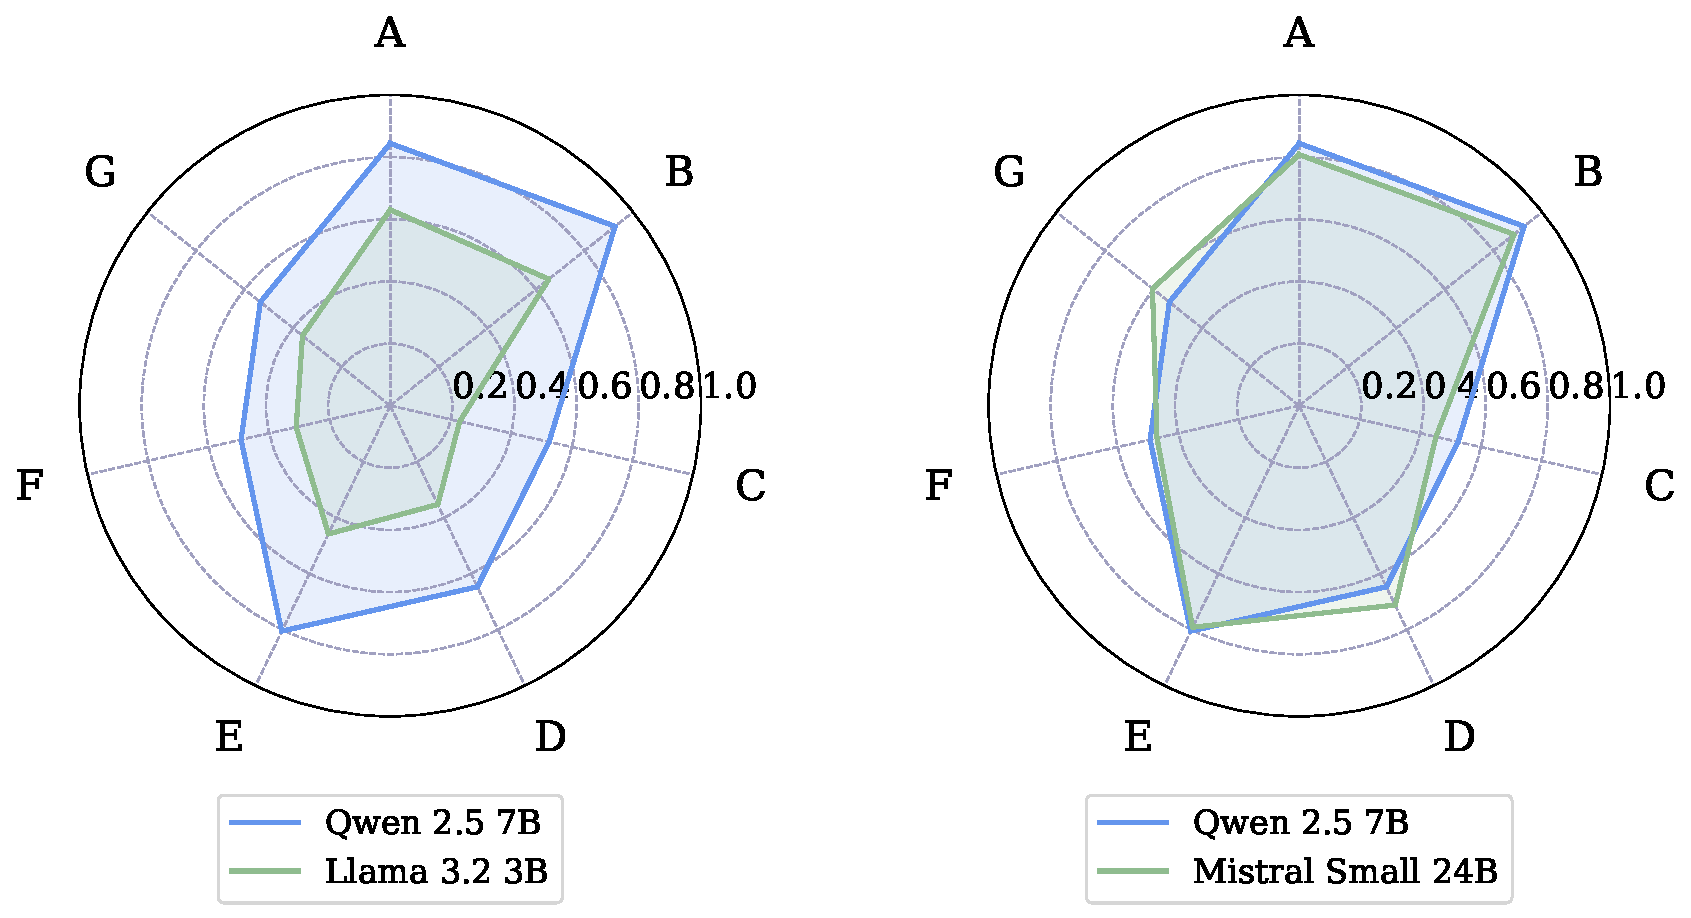
\includegraphics[width=\linewidth]{Figures/radar_compare_pairs.pdf}
    \vspace{-20pt}
    \caption{\textbf{Comparison of Model Choices}. Accuracy on 7 subjects for two model selection settings on MATH dataset. Subjects are denoted as: A = Prealgebra, B = Algebra, C = Intermediate Algebra, D = Number Theory, E = Counting \& Probability, F = Geometry, G = Precalculus.}

    \vspace{-10pt}
    \label{fig:motivation-search}
\end{wrapfigure}
% After we select the model, the next question is how much test-time compute budget should we use to wisely improve accuracy. We next scale test-time compute to further improve the accuracy. We empirically explore two dimensions for scaling compute at test time to find the best accuracy. These dimensions are described as follows:


% At a high level, given that scaling compute at test-time is a proven strategy for improving accuracy, we also explore this direction.
Next, we empirically investigate two dimensions of test-time scaling to further enhance the performance of our \NAME{}{} with selected models.

\looseness=-1
\textbf{Adding More Participating Model Types:} As we scale the model participating model types used in the system by adding more SLMs with complementary strengths, we expect the overall accuracy to improve. For each budgeted number of models, we use the search method proposed in Section~\ref{sub:method-search} to identify the best selection from the pool. 

\textbf{Drawing More Samples per Model:} For a fixed model selection, we can increase the compute budget by scaling the number of samples drawn by each model. Since confidence is evaluated by counting the frequency of majority answers, adding more samples per model is expected to provide a more accurate confidence estimate.


These two compute scaling dimensions are evaluated in Section~\ref{sub:scaling-results}.

% \label{subsub:tuning}
%  The architecture described above provides an identical prompt to each model. This "one-size-fits-all" approach is inherently limited, as it fails to account for the fact that different models have distinct strengths, weaknesses, and reasoning patterns. Therefore, prompts should be tailored to each model to leverage its specific advantages and mitigate its shortcomings.

% Instead of tuning the prompts for the entire compositional system in an end-to-end manner, we adopted an approach from prior work. We tuned the prompt for each model individually. These optimized prompts were then integrated into our \NAME{}{} framework, where each model was assigned its own tailored prompt in place of the original, uniform one.

% Specifically, we employed a genetic algorithm-inspired approach to tune the prompts. The process begins with the original uniform prompt as the initial seed. For each model, we sample an evaluation set of 25 questions from the dataset. We then iterate the following process ten times:

% First, we assess the performance of the current prompt with its corresponding model on the evaluation set. Based on the results, we generate new candidate prompts using a separate "Tuner LLM" which applies one of two strategies:

% \begin{enumerate}
%     \item \textbf{Mutation}: The Tuner LLM is provided with the current prompt, along with one correctly and one incorrectly answered question from the evaluation set, and is instructed to revise the prompt.
%     \item \textbf{Generation}: The Tuner LLM is provided only with the correct and incorrect examples and is tasked with generating an entirely new prompt from scratch.
% \end{enumerate}

% We observed that the optimal strategy (Mutation vs. Generation) is sensitive to the specific model and dataset being used. As a further detail, the models whose prompts were being tuned consistently used a sampling temperature of 0. We also experimented with using a non-zero temperature, which is a necessary condition for the multi-sample strategy in our \NAME{}{} method. However, we found that tuning prompts with multiple samples led to inconsistent impacts on final performance. Therefore, for simplicity and reproducibility, we opted to set the temperature to 0 during the prompt tuning phase.


% A key advantage of this method is that optimization occurs entirely at inference time. This avoids computationally expensive procedures like fine-tuning or retraining, which require modifying the model's weights.



